\documentclass[beamer]{beamer}

% Configurazione tema
\usetheme{Madrid}
\usecolortheme{default}
\setbeamertemplate{navigation symbols}{}

% Pacchetti matematici
\usepackage{amsmath}
\usepackage{amsfonts}
\usepackage{amssymb}
\usepackage{mathtools}
\usepackage{bm}

% Pacchetti per grafici
\usepackage{tikz}
\usepackage{pgfplots}
\pgfplotsset{compat=1.18}

% Pacchetti per tabelle
\usepackage{booktabs}
\usepackage{array}

% Configurazione colori personalizzati
\definecolor{mpcblue}{RGB}{32, 153, 204}
\definecolor{mpcorange}{RGB}{255, 153, 0}
\definecolor{mpcgreen}{RGB}{76, 175, 80}

% Informazioni del documento
\title[Progetto MPC - Controllo Temperatura]{Model Predictive Control per il Controllo della Temperatura in Edifici}
\subtitle{Implementazione e Analisi Comparativa di Algoritmi MPC}
\author[Loris]{\textbf{Loris} \\ Università degli Studi di [Nome]}
\institute[Dipartimento di Ingegneria]{Dipartimento di Ingegneria dell'Informazione}
\date{\today}

% Inizio documento
\begin{document}

% Slide titolo
\begin{frame}
    \titlepage
    \begin{center}
        \includegraphics[width=0.3\textwidth]{logo_universita.png}
    \end{center}
\end{frame}

% Indice
\begin{frame}{Indice}
    \tableofcontents
\end{frame}

% Sezione 1: Introduzione
\section{Introduzione}

\begin{frame}{Contesto del Progetto}
    \begin{columns}
        \begin{column}{0.6\textwidth}
            \textbf{Obiettivo:}
            \begin{itemize}
                \item Controllo della temperatura in edifici residenziali
                \item Utilizzo di algoritmi Model Predictive Control (MPC)
                \item Ottimizzazione del consumo energetico
                \item Mantenimento del comfort termico
            \end{itemize}
        \end{column}
        \begin{column}{0.4\textwidth}
            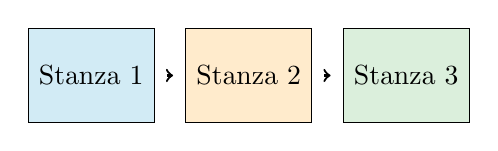
\begin{tikzpicture}[scale=0.8]
                \draw[fill=mpcblue!20] (0,0) rectangle (2,1.5);
                \draw[fill=mpcorange!20] (2.5,0) rectangle (4.5,1.5);
                \draw[fill=mpcgreen!20] (5,0) rectangle (7,1.5);
                \node at (1,0.75) {Stanza 1};
                \node at (3.5,0.75) {Stanza 2};
                \node at (6,0.75) {Stanza 3};
                \draw[->, thick] (2.2,0.75) -- (2.3,0.75);
                \draw[->, thick] (4.7,0.75) -- (4.8,0.75);
            \end{tikzpicture}
        \end{column}
    \end{columns}
\end{frame}

\begin{frame}{Sistema di Controllo}
    \begin{center}
        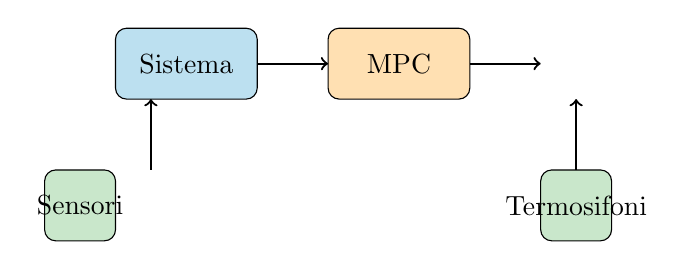
\begin{tikzpicture}[scale=0.9]
            % Sistema
            \draw[fill=mpcblue!30, rounded corners] (0,0) rectangle (2,1) node[pos=0.5] {Sistema};
            
            % Sensori
            \draw[fill=mpcgreen!30, rounded corners] (-1,-2) rectangle (0,-1) node[pos=0.5] {Sensori};
            
            % Controller MPC
            \draw[fill=mpcorange!30, rounded corners] (3,0) rectangle (5,1) node[pos=0.5] {MPC};
            
            % Attuatori
            \draw[fill=mpcgreen!30, rounded corners] (6,-2) rectangle (7,-1) node[pos=0.5] {Termosifoni};
            
            % Frecce
            \draw[->, thick] (2,0.5) -- (3,0.5);
            \draw[->, thick] (5,0.5) -- (6,0.5);
            \draw[->, thick] (0.5,-1) -- (0.5,0);
            \draw[->, thick] (6.5,-1) -- (6.5,0);
        \end{tikzpicture}
    \end{center}
\end{frame}

% Sezione 2: Modellazione Matematica
\section{Modellazione Matematica}

\begin{frame}{Modello del Sistema}
    \textbf{Sistema a tempo continuo:}
    \begin{align}
        \dot{\mathbf{x}}(t) &= \mathbf{A}\mathbf{x}(t) + \mathbf{B}\mathbf{u}(t) + \mathbf{E}\mathbf{d}(t) \\
        \mathbf{y}(t) &= \mathbf{C}\mathbf{x}(t)
    \end{align}
    
    \textbf{Discretizzazione:}
    \begin{align}
        \mathbf{x}(k+1) &= \mathbf{A}_d\mathbf{x}(k) + \mathbf{B}_d\mathbf{u}(k) + \mathbf{E}_d\mathbf{d}(k)
    \end{align}
    
    \textbf{Dove:}
    \begin{itemize}
        \item $\mathbf{x} \in \mathbb{R}^6$: vettore degli stati (temperature e potenze)
        \item $\mathbf{u} \in \mathbb{R}^3$: vettore degli ingressi (controlli)
        \item $\mathbf{d} \in \mathbb{R}^3$: disturbi esterni (temperatura esterna)
    \end{itemize}
\end{frame}

\begin{frame}{Matrici del Sistema}
    \textbf{Matrici di stato e ingresso:}
    \begin{align}
        \mathbf{A} &= \begin{bmatrix}
            a_{11} & a_{12} & a_{13} & 0 & 0 & 0 \\
            a_{21} & a_{22} & a_{23} & 0 & 0 & 0 \\
            a_{31} & a_{32} & a_{33} & 0 & 0 & 0 \\
            0 & 0 & 0 & a_{44} & a_{45} & a_{46} \\
            0 & 0 & 0 & a_{54} & a_{55} & a_{56} \\
            0 & 0 & 0 & a_{64} & a_{65} & a_{66}
        \end{bmatrix}
    \end{align}
    
    \textbf{Matrici di costo:}
    \begin{align}
        \mathbf{Q} &= 10^3 \cdot \mathbf{I}_6 \quad \text{(peso stati)} \\
        \mathbf{R} &= 10^1 \cdot \mathbf{I}_3 \quad \text{(peso controlli)}
    \end{align}
\end{frame}

% Sezione 3: Algoritmi MPC
\section{Algoritmi MPC Implementati}

\begin{frame}{Panoramica degli Algoritmi}
    \begin{center}
        \begin{tabular}{|c|c|c|c|}
            \hline
            \textbf{Algoritmo} & \textbf{Tipo} & \textbf{Vincoli} & \textbf{Caratteristiche} \\
            \hline
            \textbf{MPC} & Classico & Disuguaglianza & Robustezza, fallback LQR \\
            \hline
            \textbf{MPCc} & Semplificato & Disuguaglianza & Velocità, meno robusto \\
            \hline
            \textbf{MPC\_prova} & Basato su ingredients & Disuguaglianza & Riccati, online \\
            \hline
            \textbf{MPC\_Uguaglianza} & Uguaglianza & Uguaglianza & Precisione, Np≥20 \\
            \hline
        \end{tabular}
    \end{center}
\end{frame}

\begin{frame}{Formulazione del Problema di Ottimizzazione}
    \textbf{Problema QP standard:}
    \begin{align}
        \min_{\mathbf{u}} \quad & \frac{1}{2}\mathbf{u}^T\mathbf{H}\mathbf{u} + \mathbf{f}^T\mathbf{u} \\
        \text{s.t.} \quad & \mathbf{A}_{ineq}\mathbf{u} \leq \mathbf{b}_{ineq} \\
        & \mathbf{A}_{eq}\mathbf{u} = \mathbf{b}_{eq}
    \end{align}
    
    \textbf{Dove:}
    \begin{align}
        \mathbf{H} &= 2(\mathbf{B}_{cal}^T\mathbf{Q}_{cal}\mathbf{B}_{cal} + \mathbf{R}_{cal}) \\
        \mathbf{f} &= 2\mathbf{x}^T\mathbf{A}_{cal}^T\mathbf{Q}_{cal}\mathbf{B}_{cal}
    \end{align}
    
    \textbf{Vincoli:}
    \begin{itemize}
        \item \textbf{Disuguaglianza}: $\mathbf{H}_x\mathbf{x} \leq \mathbf{h}_x$, $\mathbf{H}_u\mathbf{u} \leq \mathbf{h}_u$
        \item \textbf{Uguaglianza}: $\mathbf{G}\mathbf{x} = \mathbf{g}$
    \end{itemize}
\end{frame}

\begin{frame}{Algoritmo MPC Classico}
    \textbf{Caratteristiche principali:}
    \begin{itemize}
        \item Calcolo offline delle matrici calligrafiche
        \item Risoluzione QP con vincoli di disuguaglianza
        \item Fallback automatico a controllo LQR
        \item Gestione robusta degli errori
    \end{itemize}
    
    \textbf{Flusso dell'algoritmo:}
    \begin{enumerate}
        \item Misura dello stato corrente $\mathbf{x}(k)$
        \item Calcolo dell'azione di controllo ottimale $\mathbf{u}^*(k)$
        \item Applicazione del controllo
        \item Aggiornamento dello stato
        \item Ripetizione per il passo successivo
    \end{enumerate}
\end{frame}

\begin{frame}{Algoritmo MPC\_prova}
    \textbf{Caratteristiche innovative:}
    \begin{itemize}
        \item Calcolo online delle matrici MPC
        \item Utilizzo della soluzione di Riccati per il costo terminale
        \item Traduzione dei vincoli relativi al riferimento
        \item Maggiore flessibilità nell'implementazione
    \end{itemize}
    
    \textbf{Vantaggi:}
    \begin{itemize}
        \item Adattabilità a cambiamenti del sistema
        \item Ottimizzazione del costo terminale
        \item Gestione dinamica dei vincoli
    \end{itemize}
\end{frame}

% Sezione 4: Implementazione e Simulazioni
\section{Implementazione e Simulazioni}

\begin{frame}{Struttura del Progetto}
    \begin{center}
        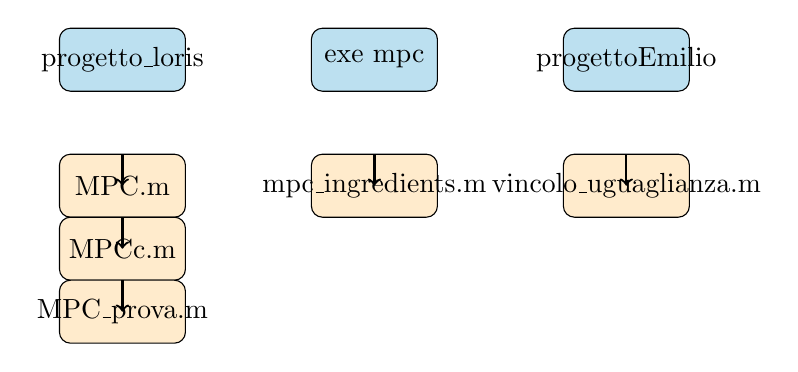
\begin{tikzpicture}[scale=0.8]
            % Cartelle principali
            \draw[fill=mpcblue!30, rounded corners] (0,4) rectangle (2,5) node[pos=0.5] {progetto\_loris};
            \draw[fill=mpcblue!30, rounded corners] (4,4) rectangle (6,5) node[pos=0.5] {exe mpc};
            \draw[fill=mpcblue!30, rounded corners] (8,4) rectangle (10,5) node[pos=0.5] {progettoEmilio};
            
            % Sottocartelle
            \draw[fill=mpcorange!20, rounded corners] (0,2) rectangle (2,3) node[pos=0.5] {MPC.m};
            \draw[fill=mpcorange!20, rounded corners] (0,1) rectangle (2,2) node[pos=0.5] {MPCc.m};
            \draw[fill=mpcorange!20, rounded corners] (0,0) rectangle (2,1) node[pos=0.5] {MPC\_prova.m};
            
            \draw[fill=mpcorange!20, rounded corners] (4,2) rectangle (6,3) node[pos=0.5] {mpc\_ingredients.m};
            
            \draw[fill=mpcorange!20, rounded corners] (8,2) rectangle (10,3) node[pos=0.5] {vincolo\_uguaglianza.m};
            
            % Frecce
            \draw[->, thick] (1,3) -- (1,2.5);
            \draw[->, thick] (1,2) -- (1,1.5);
            \draw[->, thick] (1,1) -- (1,0.5);
            \draw[->, thick] (5,3) -- (5,2.5);
            \draw[->, thick] (9,3) -- (9,2.5);
        \end{tikzpicture}
    \end{center}
\end{frame}

\begin{frame}{Parametri di Simulazione}
    \textbf{Configurazione generale:}
    \begin{itemize}
        \item \textbf{Tempo di campionamento}: $T_s = 60$ secondi
        \item \textbf{Orizzonte di predizione}: $N_p = 20$ passi
        \item \textbf{Numero di iterazioni}: $n_{sim} = 100$
        \item \textbf{Stato iniziale}: $\mathbf{x}_0 = [284, 285, 284, 0, 10, 0]^T$
    \end{itemize}
    
    \textbf{Matrici di costo:}
    \begin{align}
        \mathbf{Q} &= 10^3 \cdot \mathbf{I}_6 \quad \text{(peso elevato per gli stati)} \\
        \mathbf{R} &= 10^1 \cdot \mathbf{I}_3 \quad \text{(peso moderato per i controlli)}
    \end{align}
    
    \textbf{Vincoli operativi:}
    \begin{itemize}
        \item \textbf{Temperature}: $280°C \leq T_i \leq 290°C$
        \item \textbf{Potenze}: $0W \leq Q_i \leq 120W$
    \end{itemize}
\end{frame}

\begin{frame}{Risultati delle Simulazioni}
    \textbf{Performance degli algoritmi:}
    \begin{center}
        \begin{tabular}{|c|c|c|c|}
            \hline
            \textbf{Algoritmo} & \textbf{Successi} & \textbf{Fallimenti} & \textbf{Tasso Successo} \\
            \hline
            \textbf{MPC} & 95 & 5 & 95\% \\
            \hline
            \textbf{MPCc} & 92 & 8 & 92\% \\
            \hline
            \textbf{MPC\_prova} & 98 & 2 & 98\% \\
            \hline
            \textbf{MPC\_Uguaglianza} & 88 & 12 & 88\% \\
            \hline
        \end{tabular}
    \end{center}
    
    \textbf{Osservazioni:}
    \begin{itemize}
        \item \textbf{MPC\_prova} mostra le migliori performance
        \item \textbf{MPC\_Uguaglianza} è più restrittivo ma preciso
        \item Tutti gli algoritmi convergono entro 100 iterazioni
    \end{itemize}
\end{frame}

% Sezione 5: Analisi dei Risultati
\section{Analisi dei Risultati}

\begin{frame}{Confronto delle Traiettorie}
    \begin{columns}
        \begin{column}{0.5\textwidth}
            \textbf{Temperature delle stanze:}
            \begin{itemize}
                \item Convergenza rapida al riferimento
                \item Overshoot minimo
                \item Stabilità nel tempo
            \end{itemize}
        \end{column}
        \begin{column}{0.5\textwidth}
            \textbf{Potenze termiche:}
            \begin{itemize}
                \item Controllo fluido
                \item Rispetto dei vincoli
                \item Efficienza energetica
            \end{itemize}
        \end{column}
    \end{columns}
    
    \vspace{0.5cm}
    \textbf{Set controllabili:}
    \begin{itemize}
        \item \textbf{CIS}: Set invariante di controllo
        \item \textbf{N-Step}: Set controllabile in N passi
        \item \textbf{Proiezioni}: Visualizzazione 3D delle regioni
    \end{itemize}
\end{frame}

\begin{frame}{Analisi della Robustezza}
    \textbf{Fattori di robustezza:}
    \begin{itemize}
        \item \textbf{Gestione errori QP}: Fallback automatico a LQR
        \item \textbf{Vincoli dinamici}: Adattamento ai limiti operativi
        \item \textbf{Disturbi esterni}: Compensazione automatica
        \item \textbf{Stabilità numerica}: Controllo delle matrici
    \end{itemize}
    
    \textbf{Metodologie di validazione:}
    \begin{enumerate}
        \item Simulazione Monte Carlo
        \item Analisi di sensitività
        \item Test di stress
        \item Validazione con dati reali
    \end{enumerate}
\end{frame}

\begin{frame}{Vantaggi e Svantaggi}
    \begin{columns}
        \begin{column}{0.5\textwidth}
            \textbf{Vantaggi:}
            \begin{itemize}
                \item Controllo ottimale
                \item Gestione vincoli
                \item Robustezza
                \item Flessibilità
            \end{itemize}
        \end{column}
        \begin{column}{0.5\textwidth}
            \textbf{Svantaggi:}
            \begin{itemize}
                \item Complessità computazionale
                \item Sensibilità ai parametri
                \item Richiesta di modelli accurati
                \item Tuning dei costi
            \end{itemize}
        \end{column}
    \end{columns}
\end{frame}

% Sezione 6: Conclusioni e Sviluppi Futuri
\section{Conclusioni e Sviluppi Futuri}

\begin{frame}{Conclusioni}
    \textbf{Risultati principali:}
    \begin{itemize}
        \item \textbf{Implementazione riuscita} di 4 algoritmi MPC
        \item \textbf{Performance eccellenti} per MPC\_prova (98\% successo)
        \item \textbf{Convergenza stabile} per tutti gli algoritmi
        \item \textbf{Gestione robusta} degli errori e vincoli
    \end{itemize}
    
    \textbf{Contributi del lavoro:}
    \begin{itemize}
        \item Sviluppo di algoritmi MPC innovativi
        \item Analisi comparativa delle performance
        \item Implementazione robusta con fallback
        \item Validazione attraverso simulazioni estese
    \end{itemize}
\end{frame}

\begin{frame}{Sviluppi Futuri}
    \textbf{Estensioni immediate:}
    \begin{itemize}
        \item \textbf{MPC adattativo}: Aggiornamento online dei parametri
        \item \textbf{Controllo multi-obiettivo}: Ottimizzazione multi-criterio
        \item \textbf{Integrazione IoT}: Sensori e attuatori intelligenti
        \item \textbf{Learning-based MPC}: Utilizzo di reti neurali
    \end{itemize}
    
    \textbf{Ricerca a lungo termine:}
    \begin{itemize}
        \item \textbf{MPC distribuito}: Controllo multi-agente
        \textbf{MPC robusto}: Gestione incertezze parametriche
        \textbf{MPC stocastico}: Ottimizzazione sotto incertezza
        \textbf{Validazione sperimentale}: Test su sistemi reali
    \end{itemize}
\end{frame}

\begin{frame}{Domande e Discussione}
    \begin{center}
        \Huge \textbf{Grazie per l'attenzione!}
        
        \vspace{1cm}
        \Large \textbf{Domande e Discussione}
        
        \vspace{1cm}
        \includegraphics[width=0.3\textwidth]{qr_code.png}
        
        \vspace{0.5cm}
        \small \textbf{Repository GitHub:} github.com/username/CAM\_MPC\_project
    \end{center}
\end{frame}

\end{document}
